\documentclass{article} \usepackage[utf8]{inputenc}
\usepackage{amsmath, amssymb, systeme, mathtools, lmodern, float, graphicx, multicol, titlesec, listings}
\usepackage[dvipsnames]{xcolor}
\usepackage[scale=.95,type1]{cabin}
\usepackage[framemethod=tikz]{mdframed}

\usepackage[legalpaper,margin=1in]{geometry}

\setlength{\parindent}{10pt}
% \setlength{\parskip}{1em}
\renewcommand{\baselinestretch}{1.2}


\definecolor{codegreen}{rgb}{0,0.6,0}
\definecolor{codegray}{rgb}{0.5,0.5,0.5}
\definecolor{backcolour}{rgb}{0.93725490196,0.94509803921,0.96078431372}
\definecolor{codewhite}{rgb}{0.75,0.78,0.84}
\definecolor{normalcode}{rgb}{0.35,0.36,0.45}

\lstdefinestyle{mystyle}{
    backgroundcolor=\color{backcolour},   
    commentstyle=\color{codegray},
    keywordstyle=\color{magenta},
    numberstyle=\small\color{codegray}\fontfamily{cmtt}\selectfont,
    stringstyle=\color{codegreen},
    basicstyle=\ttfamily\color{normalcode},
    breakatwhitespace=false,         
    frame=single,
    breaklines=true,                 
    captionpos=b,                    
    keepspaces=true,                 
    numbers=left,                    
    numbersep=5pt,                  
    showspaces=false,                
    showstringspaces=false,
    showtabs=false,                  
    tabsize=2
}

\lstset{style=mystyle}
\title{LESS AD-HOC POLYMORPHISM}
\date{}
\author{}

\newcounter{Def}[section]
\newenvironment{Def}[1][]{%
  \ifstrempty{#1}%
  {\mdfsetup{%
    frametitle={%
      \tikz[baseline=(current bounding box.east),outer sep=0pt]
      \node[line width=1pt,anchor=east,rectangle,draw=blue!20,fill=white]
    {\strut \color{black}{Definition}~};}}
  }%
  {\mdfsetup{%
    frametitle={%
      \tikz[baseline=(current bounding box.east),outer sep=0pt]
      \node[line width=1pt,anchor=east,rectangle,draw=Lavender!20,fill=white]
    {\strut ~\color{RubineRed!60}{#1}};}}%
  }%
  \mdfsetup{innertopmargin=2pt,linecolor=Lavender!20,%
            linewidth=1pt,topline=true,%
            frametitleaboveskip=\dimexpr-\ht\strutbox\relax,}
  \begin{mdframed}[]\relax%
  }{\end{mdframed}}

\titleformat{\section}
  {\fontfamily{lmss}\selectfont\LARGE\color{black}}
  {\thesection}{1em}{}
\begin{document}
  \maketitle
   Unlike other languages, Haskell does not provide universal stringification (Show/ print)
   or equality (Eq (value equality)) ...

   \section{Type-defaulting typeclasses}
\begin{minipage}[]{0.4\linewidth}
\begin{center} 
 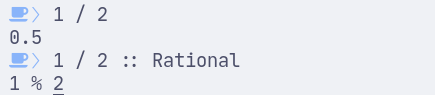
\includegraphics[width=6.5 cm]{img/2022-08-31-13-35-31.png}
 \end{center} 
\end{minipage}
\begin{minipage}[]{0.57\linewidth}
   When evaluate a \textit{polymorphic value}, the polymorphism must be resolved to a
   specific \textbf{concrete type}. For example, this is set to {\fontfamily{cmtt}\selectfont Double} by default.
\end{minipage}

   \begin{Def}[Typeclass inheritance]
       Typeclass inheritance is when a typeclasses has a \textbf{superclass}.
       A typeclasses requires another typeclasses to be available for a given
       type before you can write an instance.
   \end{Def}

   \begin{multicols}{2}
\begin{itemize} \renewcommand\labelitemi{\small \textcolor{Lavender}{$\blacksquare$}}
  \item \textbf{Effects:} are how we refer to \textit{observable} action programs may take than compute a value.
  \item \textbf{Instance:} the definition of how a typeclass should work for a given type. 
\end{itemize}
   \end{multicols}

   Running {\fontfamily{cmtt}\selectfont main} \textit{only} produce side effects. Its type must be {\fontfamily{cmtt}\selectfont IO ()}.

   \section{Typeclass inheritance, partial}
\begin{center} 
 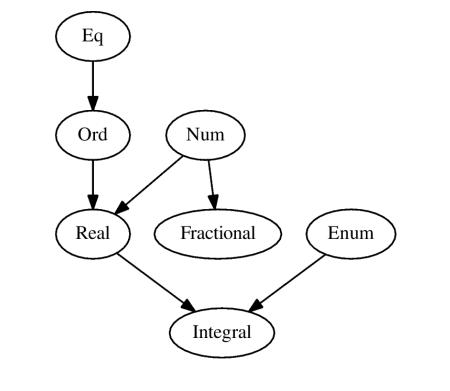
\includegraphics[width=8 cm]{img/2022-09-02-16-28-27.png}
 \end{center} 
   % \lstinputlisting[language=Haskell]{./207.hs}



\end{document}
